\documentclass[]{./assets/tex/report-template}
\usepackage{graphicx}
\usepackage{listings}
\usepackage{hyperref}
\hypersetup{
    colorlinks=true,
    linkcolor=blue,
    filecolor=magenta,      
    urlcolor=cyan,
}
\lstset{
    mathescape=true,
    basicstyle = \ttfamily
}
\usepackage[backend=biber,style=nature]{biblatex}
\addbibresource{./assets/tex/bibliography.bib}


%%%%%%%%%%%%%%%%%%%%%%
%%% Cover Page

\def\studentname{Rajit Banerjee}
\def\studentid{18202817}
\def\projecttitle{Performance Analysis of Design Patterns in Microservice Architecture}
\def\supervisorname{Professor John Murphy}

\begin{document}
\maketitle

%%%%%%%%%
%\tableofcontents

%%%%%%%%%
%\abstract
%Provide a short description here (about 150-200 words) of your project. Do not go into fine detail, but offer a strategic overview of the project’s aims. An abstract should whet the appetite for what comes next, not quench it with details.


%%%%%%%%
\section{Initial Project Specification}

\subsection{Problem Statement}
Microservice architecture is a style of designing software systems to be highly maintainable, scalable, loosely-coupled and independently deployable. Moreover, each service is built to be self-contained and implement a single business capability. Design patterns in software engineering refer to any general, repeatable or reusable solution to recurring problems faced during the software design process. The aim of this project is to study the performance engineering practices associated with a number of \textit{microservice design patterns}, considering both qualitative and quantitative metrics to evaluate their benefits and shortcomings depending on the business requirement and use case. A non-exhaustive list of design patterns that could be explored is as follows:

\begin{itemize}
	\item API Gateway
	\item Asynchronous Messaging
	\item Chain of Responsibility
	\item Database or Shared Data
	\item Circuit Breaker
	\item Externalise Configuration
	\item Aggregator
	\item Branch
\end{itemize}

Employing some of the aforementioned design patterns, sufficiently complex simulations will be designed for the performance engineering experiments. The project will also look at some common issues in microservices, and how they compare with traditional monolithic architectures.

\subsection{Background}
Microservices have gained traction in recent years with the rise of Agile software development and a DevOps \cite{awsDevOps} approach. As software engineers migrate from monoliths to microservices, it is important to make appropriate choices for system design and avoid "anti-patterns". Although no one design pattern can be called the "best", the performance of systems can be optimised by following design patterns suited to the use case, with the right configuration of hardware resources.

\subsection{Related Work}
Due to their popularity, microservices have been written about extensively in books like \cite{richardson18}, \cite{kleppmann17}, \cite{newman14}. Articles such as \cite{md19}, \cite{md20}, \cite{sahiti20}, \cite{udantha19}, \cite{lewis14} discuss the intricacies of microservice architecture as well as the trade-offs between various common design patterns. In \cite{cully20}, the performance problems inherent to microservices are explored, with evaluations performed using a custom-built prototyping suite. Akbulut and Perros \cite{akbulut19} dive into the performance analysis aspect of microservices that is being proposed in this project, where they consider 3 different design patterns.

\subsection{Datasets}
Any data that is to be used or analysed in this project will be generated during the course of experiments. There are no dependencies on additional datasets.

\subsection{Resources Required}
A non-exhaustive list of resources is specified below, following preliminary needs assessment.

\begin{itemize}
	\item Languages/Frameworks: Java, Spring Boot, Python
	\item Tools: Git, Docker, Apache JMeter
	\item Database: MongoDB
	\item Compute: Linux server maintained by the UCD School of Computer Science
\end{itemize}



%%%%%%%%%
%\chapter{Introduction}

TODO Introduce your vision of the project here. Describe the domain of the project, and the intended application. A well-written report will answer three key questions: What am I doing in this project? Why is it worth doing? How do I plan to go about it? In this introductory section, offer a concise answer to the What, and follow-up with a compelling account of the Why. Leave the How to a subsequent section. Do not try to do too much in any single section of the report. By providing details in a logical order, you will show that you have a plan for the report and the project.


%%%%%%%%%
%\chapter{Related Work and Ideas}

A key task of this first report is to establish a baseline against which your later work will be judged. Your FYP project does not exist in a vacuum, and its central problem, or a variant thereof, will have been tackled by others before you. In this section, you should describe how previous approaches have tackled the problem, and clearly articulate the state of the art (or SOA) for your project.

For research-oriented projects, this task will be time-consuming but relatively straightforward. You should read past works on the subject, summarise the main points, pros and cons, and root out the previous works that they cite in turn. You may use Wikipedia as a secondary source only, which is to say that it can be a useful first port of call on many topics but not a source that should be liberally cited. Rather, use Wikipedia as a hub for gathering references to primary work in the field (original papers and reports), then read and summarise those. Do not quote a work that you have not read, unless you are quoting someone else’s view of that work. Never use another writer’s words as your own. Place any extracts from another’s work in double quotes, and attribute the quotation to its author with a citation. It is a very low act to plagiarise another’s work and take credit for their words, so tread carefully. Even unintentional plagiarism is still plagiarism.

For more application-oriented projects, you are still expected to survey other solutions, either for the given problem or for similar problems, and also consider applications that share functionality or design principles with your own. In short, this section is the core of your report regardless of what kind of project you do.


%%%%%%%%%
%\chapter{Data Considerations}

In this section you should characterise the nature and scale of the data you are working with. Outline the shape of the data, where you expect to obtain it, and the size of the data. Is it static or dynamic, local or remote, stored or streaming? Is it raw or structured? Is it unfiltered user data, or is it curated by a specialist? What is your rationale for using this data and not other data? If your project looks at callout times for Spanish ambulances, usage rates of French parking lots, alcohol consumption in Germany, and so on, then explain why you are not using Irish data for the project. Indicate the data-cleaning processes that you anticipate will be necessary. What licensing restrictions, if any, apply to your data? Will you be making this data public after your project is completed? Are there any privacy or ethical issues with how the data is to be collected or used? If so, discuss here.

Some or many of these questions may be moot in the case of specific projects, but you should provide compelling answers to any that seem relevant. Since this provides the foundation for your project, your reviewers will be looking closely.


%%%%%%%%%
%\chapter{Outline of Approach}

In order to demonstrate various performance engineering practices in the context of microservice design patterns, we look at a simple movie ticket reservation system, consisting of 3 independent cinemas (Cineworld, Dundrum and UCD), as well as an intermediary (or broker) between clients and the cinema services. Each cinema has its own catalogue of movies (with an ID, name, and available showtimes). The client's primary objective would be to request the intermediary to fetch a list of movies from every active cinema, then display aggregated results. Next, the client selects a movie and showtime (along with other booking details) to make a reservation at a specific cinema. It is also possible to list the reservations made at a given cinema (useful for staff and administrators). The intermediary serves as a router for client requests to the cinema services, and in some cases, an aggregator of results.


\begin{figure}[H]
  \centering
  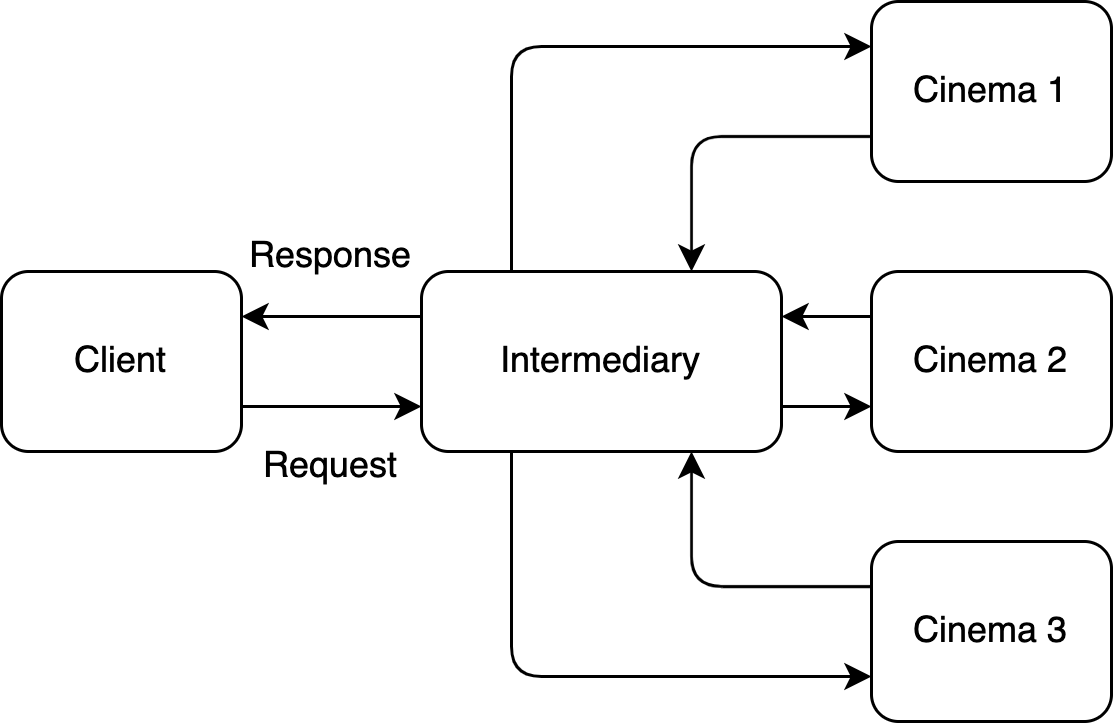
\includegraphics[width=0.5\linewidth]{./assets/diagrams/outline-arch.png}
  \caption{Prototype of movie ticket reservation system using microservices.}
  \label{fig:outline-arch}
\end{figure}


In this project, two separate web applications have been designed to model the same system described above, each employing a variety of common design patterns. The applications follow microservice architecture, with the intermediary and cinema services all being self-contained, loosely-coupled and independently deployable. Taking each application to be a \textit{case study}, the next chapter provides descriptions of the system design, implementation specifics, design pattern choices, and the associated performance implications. In a larger scale production system, it is likely that each independent cinema would in turn comprise a number of microservices to serve more specific purposes, but to avoid over-complicating the architecture in this project, cinemas are designed to be single entities.

One of the main benefits of microservices is the freedom of choice regarding the programming language used for development, since any suitable language may be used as long the service exposes an API \footnote{\url{https://www.mulesoft.com/resources/api/what-is-an-api}} adhering to known standards (typically HTTP \footnote{\url{https://developer.mozilla.org/en-US/docs/Web/HTTP}} and REST \footnote{\url{https://en.wikipedia.org/wiki/Representational_state_transfer}}). The API is then used for inter-service communication. For the case studies in this project, Java and Spring \footnote{\url{https://spring.io}} are chosen over other languages and frameworks primarily due to the dominance of Java in enterprise-level software, as well as the feature richness of Spring. Moreover, as shown in a 2017 study by Pereira et al. \cite{pereira17}, Java ranks much higher in terms of time, memory and energy efficiency; which need to be considered when talking about system performance; compared to other popular languages such as Python or TypeScript/JavaScript. The Spring framework in Java offers a plethora of integrations and abstractions to implement microservice and cloud-related design patterns, through projects such as Spring Boot, Spring Data, Spring Cloud and Spring AMQP, to name a few that are used in the case study web applications here. Apache Maven \footnote{\url{https://maven.apache.org}} is the tool used for dependency management for Java.

Each web application exposes APIs for its microservices, whose endpoints can be invoked with HTTP requests like GET and POST. In commercial systems, a website (UI client) would invoke the backend API to perform actions, but for our case studies, it is sufficient to use a tool such as Postman \footnote{\url{https://www.postman.com}} or VS Code's REST Client \footnote{\url{https://marketplace.visualstudio.com/items?itemName=humao.rest-client}} to demonstrate the API functionalities locally.

In line with industry standards, Docker \footnote{\url{https://www.docker.com}} is the infrastructure/containerisation tool used to deploy the fleet of microservices. According to Docker, Inc., a \textit{container image} is a lightweight, standalone, executable package of software that includes everything needed to run an application: code, runtime, system tools, system libraries and settings. Using Docker provides a number of advantages such as ease of standardisation, compatibility, maintainability, CI/CD, resource and application isolation, and much more. Container deployment and application testing is performed on an Ubuntu 18.04 LTS compute server (\textit{dunnion}, maintained by the UCD School of Computer Science \footnote{\url{https://www.ucd.ie/cs/}}), with a 10 core Intel(R) Xeon(R) Silver 4114 CPU (base frequency: 2.20 GHz), and 125GB system memory.

\textbf{TODO paras on performance testing/benchmarking}

%%%%%%%%%
%\chapter{Project Work Plan}

\begin{figure}[h]
	\centering
	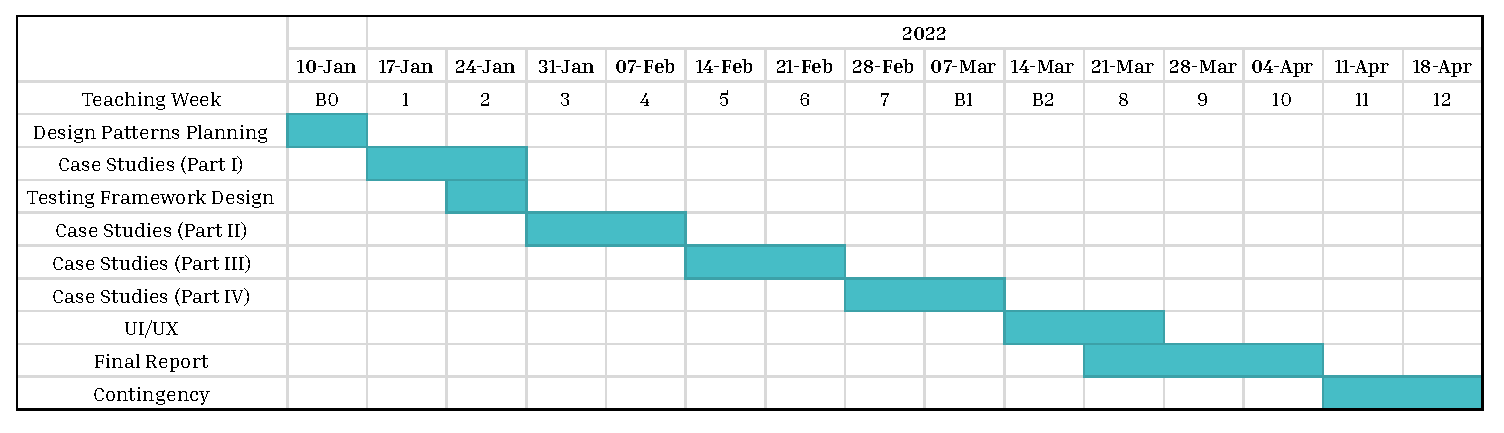
\includegraphics[width=1.0\linewidth]{./assets/images/work-plan-gantt.pdf}
	\caption{Gantt chart for project timeline}
	\label{fig:work-plan-gantt}
\end{figure}

\begin{itemize}
	\item \textbf{Design Patterns Planning (1 week)}: The initial planning here is of particular significance and will decide the direction and pace of the project's implementation phase. Various microservice design patterns will be considered to select a few important patterns which can be easily demonstrated using simulations, and then performance tested.

	\item \textbf{Testing Framework Design (1 week)}: Designing a simple testing framework (e.g. load testing plans) during the first case study will facilitate the adoption of similar strategies for subsequent case studies. 

	\item \textbf{Case Studies (Parts I, II, III, IV) (8 weeks)}: These case studies will form the bulk of the project, and will be split into four parts for convenience, each comprising a set of related design patterns (each group of case studies will possibly address 2-3 patterns). The majority of effort required here will be concerned with the back-end development of dummy microservice-based systems using containers (Docker). Evaluation, both qualitative and quantitative, is well integrated with the implementation phase of the project, since performance analysis/testing will be carried out in tandem with the case study experiments. Different configurations used during performance testing will facilitate the discussion around suitability and aptness of a number of microservice design patterns.

	\item \textbf{UI/UX (2 weeks)}: A simple web user interface will be designed to visualise the results of performance testing conducted for microservices during the different case studies, and also provide a cost-benefit analysis of the design patterns under investigation.

	\item \textbf{Final Report (3 weeks)}: Although the core parts of the report should be written as progress is made with tasks, a dedicated period is set aside for refinement and completion.

	\item \textbf{Contingency (2 weeks)}: Time set aside to be used only in the event of unforeseen issues or challenges.
\end{itemize}



%%%%%%%%%
%\chapter{Summary}

TODO: Include: key takeaways from experiments and performance analysis, future work and improvements, reflection (lessons learnt)

\section{Conclusions}

TODO

\section{Future Work}

TODO

\section{Reflection}

TODO

In this section you will sum up your report, draw some conclusions about your work so far, and make some
general observations about the work to come. You may also use this opportunity to express points of view,
or make factual claims, that are more pertinent here than in other sections of the report. If your project
raises some ethical concerns, for example about how data or users are treated, then address them here in a
thoughtful manner.

Regarding this document, here are some concluding points that you should keep in mind when writing your own.
You may use screenshots in your report, but do not overfill your report with them, or with figures of any kind.
Make sure that figures earn their keep, and are not just present as space fillers or as eye candy. If you use
diagrams or figures from other people’s work, including the web, be sure to cite the creator in the corresponding
caption. All things being equal, it is better to construct your own figures than to copy and paste those of others.
In any case, always make sure that your images are readable, do not suffer from pixelation or aliasing effects,
and that each is clearly numbered, captioned and meaningfully referenced in the main body of the text.

Ensure that there is a cohesive argument expressed in the text of the report and that it is not simply a bag of
diagrams, screenshots and wishful thinking. Every report should tell a story, so know what story you want to tell.
When you include images, make sure they are readable and truly add to the discussion.

Make sure your language is professional throughout, and steer a course between pompous and colloquial. Maintain
authorial distance and do not overuse “me,” “I” and “our.” Your are writing for a professional audience who will
judge you on the quality of your prose, so use a grammar and a spelling checker.

Use LaTeX if you wish - this is recommended if you plan to use mathematical formulae in your report, but in any
case, keep the general spacing and font/style you find here (Single or 1.5 spacing, 12 pt. font for text, etc.).
Be sure to submit a PDF (never a .DOC or .DOCX file) as your report. If you prepare your report in MS Word, as
this document has been, save it as a PDF before you submit it. Overall it should be about 18 - 20 pages, including
figures, front matter and references, A significant portion of the report will be textual, with approx.. five or
six thousand words. Do not rely on images or other filler to write your report for you.
The dates and means of submission will be communicated to you separately.


%%%%%%%%%
%\chapter{Latex Pointers}

TODO remove.

This chapter contains some examples on the usage of latex. Do not include in your final report.

\section{Figures}
From time to time, it's necessary to add pictures to your documents. Using LaTeX all pictures will be indexed automatically and tagged with successive numbers when using the figure environment and the graphicx package. We can reference the figure below using its label like this: Fig. \ref{fig:test_plot}.
\begin{figure}[H]
  \centering
  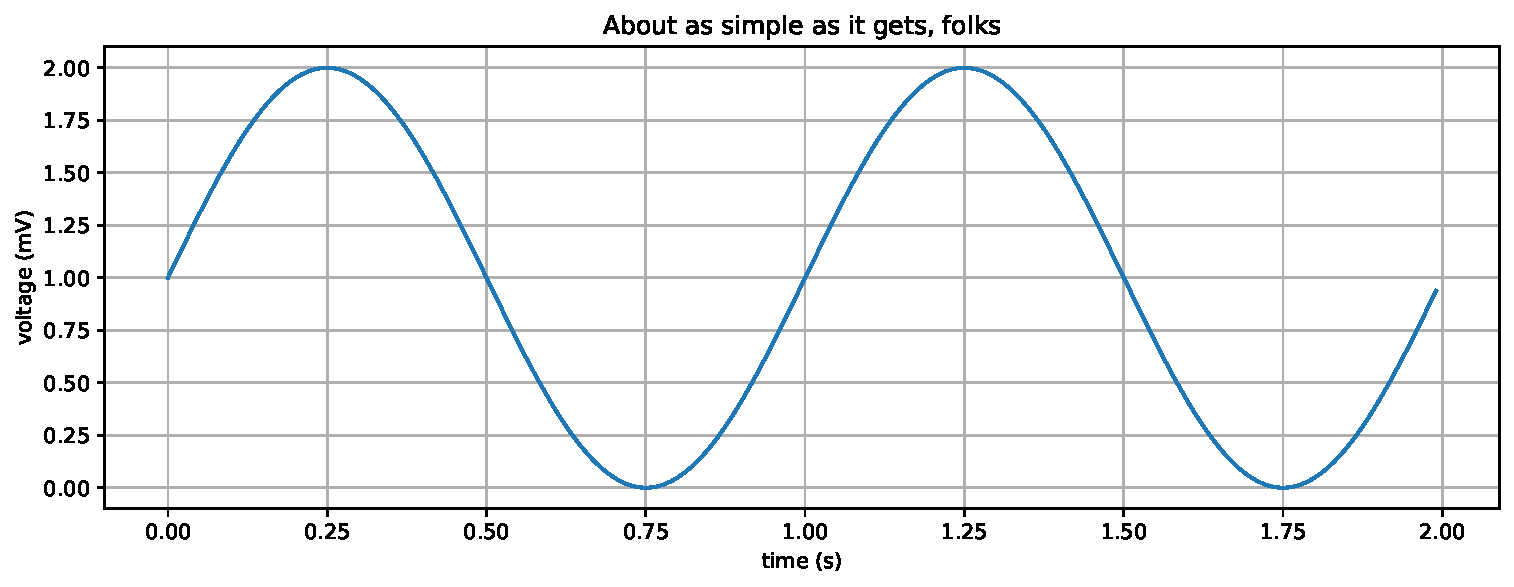
\includegraphics[width=0.8\linewidth]{./assets/images/test-plot.pdf}
  \caption{A sample graph}
  \label{fig:test_plot}
\end{figure}

Lots more information in this \href{https://www.latex-tutorial.com/tutorials/figures/}{tutorial}.


\section{Code Listing}
You can list code using the \emph{listings} package:

\begin{lstlisting}[language=Python,caption=Borg Pattern]
class Borg(object):
    __shared_state = {}

    def __init__(self):
        self.__dict__ = self.__shared_state
        self.state = 'Init'

    def __str__(self):
        return self.state
\end{lstlisting}

Lots more examples \href{https://www.overleaf.com/learn/latex/Code_listing}{here}.

\section{Math}
Here \ref{eq:limit} is an example of including an equation
\begin{equation}
  \lim_{x\to\infty} f(x)
  \label{eq:limit}
\end{equation}

More examples \href{https://www.latex-tutorial.com/tutorials/amsmath/}{here} and \href{https://www.overleaf.com/learn/latex/Mathematical_expressions}{here}.



\section{References}
Look up the bibtex references on google scholar or import from Mendeley or other reference managers. Add the bibtex snippet to the \emph{references.bib} file. Then cite the reference like this:

As explained in \cite{knuth2014art}, we also find that...

Lots more details \href{https://www.latex-tutorial.com/tutorials/bibtex/}{here}.


%%%%%%%%%
%\chapter*{Acknowledgements}

I would like to express my sincere gratitude towards:
\begin{itemize}
  \item Professor John Murphy, my project supervisor, for his guidance, support and understanding throughout the project.
  \item Associate Professor Rem Collier, for sharing his knowledge and experience with distributed systems and technologies.
  \item My team (Ulysses - Enterprise Engineering) at Amazon Web Services (Dublin), for introducing me to the world of microservice architecture.
  \item UCD School of Computer Science, for providing access to a Linux compute server.
  \item My family and friends - especially Sharon Farrell, Ciara Murphy and Alexander Bourke, for their constant encouragement.
\end{itemize}



%%%%%%%%
\printbibliography

%%%%%%%%
\end{document}
